\documentclass{beamer}
\usetheme{Madrid}
\usecolortheme{default}

% Paquetes necesarios
\usepackage[utf8]{inputenc}
\usepackage[spanish]{babel}
\usepackage{amsmath}
\usepackage{amsfonts}
\usepackage{amssymb}
\usepackage{graphicx}

% Información del título
\title{Multiplicadores de Lagrange}
\subtitle{Optimización Agrícola en el Valle del Mantaro}
\author{RONALDO CARLOS MAMANI MENA\\ YONHEL MAMANI CRUZ\\ ALEXANDER QUISPE HOLGUIN}
\institute{Universidad Nacional Del Altiplano}
\date{\today}

\begin{document}

% Diapositiva 1: Título
\frame{\titlepage}

% Diapositiva 2: Planteamiento del Problema
\begin{frame}
\frametitle{Planteamiento del Problema}
\framesubtitle{Optimización Agrícola en el Valle del Mantaro, Perú}

\begin{block}{Situación}
Un agricultor tiene \textbf{120 hectáreas} para cultivar papa y maíz
\end{block}

\begin{columns}
\begin{column}{0.5\textwidth}
\textbf{Datos económicos:}
\begin{itemize}
\item Papa: 8,000 soles/ha
\item Maíz: 6,000 soles/ha
\item Costo papa: $50x^2$ soles
\item Costo maíz: $40y^2$ soles
\end{itemize}
\end{column}
\begin{column}{0.5\textwidth}
\textbf{Problema de optimización:}
\\[0.3cm]
\textbf{Maximizar:}
$$f(x,y) = 8000x + 6000y - 50x^2 - 40y^2$$
\\[0.2cm]
\textbf{Sujeto a:}
$$x + y = 120$$
\end{column}
\end{columns}

\end{frame}

% Diapositiva 3: Método de Solución
\begin{frame}
\frametitle{Método de Multiplicadores de Lagrange}

\begin{block}{Lagrangiano}
$$L(x,y,\lambda) = 8000x + 6000y - 50x^2 - 40y^2 - \lambda(x + y - 120)$$
\end{block}

\begin{block}{Condiciones de Primer Orden}
\begin{align}
\frac{\partial L}{\partial x} &= 8000 - 100x - \lambda = 0 \quad (1)\\
\frac{\partial L}{\partial y} &= 6000 - 80y - \lambda = 0 \quad (2)\\
\frac{\partial L}{\partial \lambda} &= -(x + y - 120) = 0 \quad (3)
\end{align}
\end{block}

\end{frame}

% Diapositiva 4: Resolución del Sistema
\begin{frame}
\frametitle{Resolución del Sistema}

\begin{block}{Paso 1: Igualar las ecuaciones (1) y (2)}
De (1): $\lambda = 8000 - 100x$ \\
De (2): $\lambda = 6000 - 80y$ \\[0.2cm]
Igualando: $8000 - 100x = 6000 - 80y$ \\
Simplificando: $y = 1.25x - 25$
\end{block}

\begin{block}{Paso 2: Sustituir en la restricción}
$x + y = 120$ \\
$x + (1.25x - 25) = 120$ \\
$2.25x = 145$ \\
$x = 64.44$ hectáreas (papa)
\end{block}

\begin{block}{Paso 3: Encontrar y y $\lambda$}
$y = 120 - 64.44 = 55.56$ hectáreas (maíz) \\
$\lambda = 8000 - 100(64.44) = 1,556$ soles/hectárea
\end{block}

\end{frame}

% Diapositiva 5: Resultados
\begin{frame}
\frametitle{Resultados de la Optimización}

\begin{columns}
\begin{column}{0.5\textwidth}
\begin{block}{Solución Óptima}
\begin{itemize}
\item \textbf{Papa:} 64.44 ha (54\%)
\item \textbf{Maíz:} 55.56 ha (46\%)
\item \textbf{$\lambda^*$:} 1,556 soles/ha
\end{itemize}
\end{block}
\end{column}
\begin{column}{0.5\textwidth}
\begin{block}{Utilidad Máxima}
\begin{itemize}
\item \textbf{Ingresos:} 848,880 soles
\item \textbf{Costos:} 331,098 soles
\item \textbf{Utilidad neta:} \textcolor{red}{517,782 soles}
\end{itemize}
\end{block}
\end{column}
\end{columns}

\vspace{0.5cm}

\begin{alertblock}{Verificación}
Restricción: $64.44 + 55.56 = 120$ ✓ \\
Condiciones de optimalidad satisfechas ✓
\end{alertblock}

\end{frame}

% Diapositiva 6: Interpretación Económica
\begin{frame}
\frametitle{Interpretación Económica}

\begin{block}{Significado del Multiplicador $\lambda = 1,556$ soles/hectárea}
\begin{itemize}
\item Representa el \textbf{valor marginal} de una hectárea adicional
\item Si tuviera 121 hectáreas, la utilidad aumentaría en $\approx$ 1,556 soles
\item Es el \textbf{precio sombra} de la tierra en el Valle del Mantaro
\end{itemize}
\end{block}

\begin{block}{Recomendaciones para el Agricultor}
\begin{enumerate}
\item Destinar 54\% de tierra a papa y 46\% a maíz
\item Considerar arrendar tierra adicional si cuesta < 1,556 soles/ha/temporada
\item La diversificación reduce riesgos climáticos de la sierra peruana
\end{enumerate}
\end{block}

\begin{center}
\textbf{¡La optimización matemática maximiza la rentabilidad agrícola!}
\end{center}

\end{frame}
% Diapositiva 6: GRAFICOS
\begin{frame}
\frametitle{Graficos de la optimizacion de la Optimización}
\begin{figure}[h]
\centering
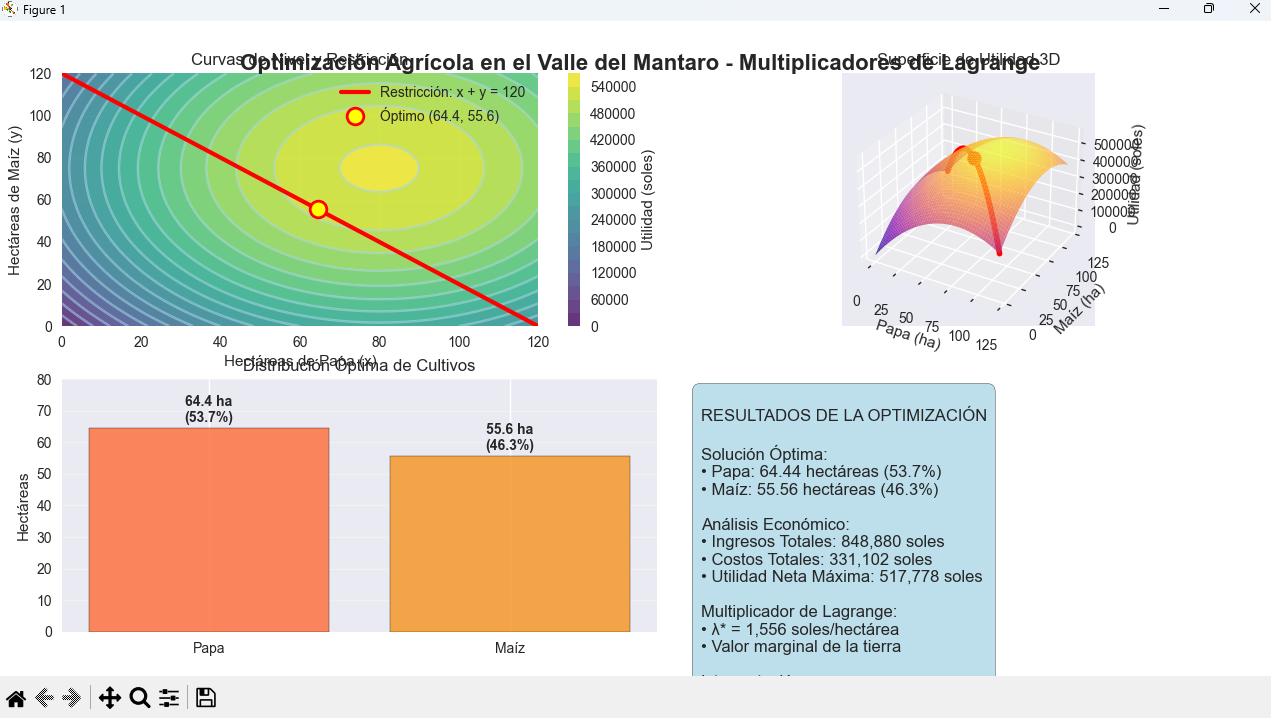
\includegraphics[width=0.8\textwidth]{SGBD_II/02_06METODOPTIM/metod.png}
\end{figure}
\end{frame}

\end{document}